% !TEX encoding = UTF-8 Unicode
\documentclass{article}
\usepackage[utf8]{inputenc}
\usepackage[table]{xcolor}
\usepackage{xurl}
\usepackage{listings,natbib}
\usepackage{hyperref,vwcol,tabularx,graphicx,multicol,xcolor,bookmark}
\title{Documentación de Catch You!}
\author{Jose_Varela}
\date{12 de junio del 2023}

% Unas cuantas configuraciones
\graphicspath{ {./} }

%%%%%%
\definecolor{codered}{rgb}{0.6,0,0}
\definecolor{codegreen}{rgb}{0,0.5,0}
\definecolor{codegray}{rgb}{0.5,0.5,0.5}
\definecolor{codeblue}{rgb}{0.3,0.3,1}
\definecolor{codepurple}{rgb}{0.58,0,0.82}
\definecolor{backcolour}{rgb}{0.95,0.95,0.92}


% There's no GDSscript language definition in LaTeX, so I have to create my own weeeeeeeeeeee
\lstdefinelanguage{GDScript}{
    % Reserved words
    morekeywords = [1]{
        func, var, return, while, for, in, if, self, break, new,
        continue, signal, not, bool, false, true, void, null, const,
        class, float, int
    },
    % Variable types
    morekeywords = [2]{
        Vector2,
        Vector2i,
        CharacterBody2D,
        CharacterBody3D,
        Dictionary,
        Array,
        PackedVector2Array,
        TileMap,
        String,
        % Custom nodes for the game
        BPSNode,
        GRNode,
        STRNode,
        \$Jugador,
        \$Interfaz
    },
    % Function names
    morekeywords = [3] {
        somethingerfhru,
        local_to_map,
        map_to_local,
        pop_front,
        search,
        getPositionAsTile,
        append,
        is_empty,
        loadfile,
        connect,
        connectMap,
        randomize,
        set_process,
        emit_signal,
        is_in_group,
        play,
        set_visible,
        stop,
        create_timer,
        save,
        set_text,
        failPlayer,
        applyShake,
        h_calc,
        length,
        getPositionTileFromMap,
        has,
        expand,
        clear,
        distance_to,
        size
    },
    keywordstyle = [1]\color{codered},
    keywordstyle = [2]\color{codegreen},
    keywordstyle = [3]\color{codeblue},
    sensitive=true, % keywords are not case-sensitive
    morecomment=[l]{\#}, % l is for line comment
    morecomment=[s]{/*}{*/}, % s is for start and end delimiter
    morestring=[b]" % defines that strings are enclosed in double quotes
} % 

\lstdefinestyle{mystyle}{
    language={GDScript},
    backgroundcolor=\color{backcolour},   
    commentstyle=\color{codegreen},
    keywordstyle=\color{magenta},
    numberstyle=\tiny\color{codegray},
    stringstyle=\color{codepurple},
    basicstyle=\ttfamily\footnotesize,
    frame={tb},
    breakatwhitespace=false,         
    breaklines=true,                 
    captionpos=b,                    
    keepspaces=true,                 
    numbers=left,                    
    numbersep=5pt,                  
    showspaces=false,                
    showstringspaces=false,
    showtabs=false,                  
    tabsize=4
}

\lstset{style=mystyle}
%%%%%%

% Comandos especificos para definir el tipo de clase que estamos.
\newcommand{\matricula}{S18001413}

\setcounter{page}{1}
\makeatletter

\def\@maketitle{
  %\begin{vwcol}[widths={0.4,0.6}, sep=.0cm, justify=flush, rule=0pt, indent=1em]
		% El logotipo es común, asi que solamente necesitamos
		% una versión del gráfico.
  \begin{center}
    \let \footnote \thanks
        { 
\includegraphics[width = 100mm]{_logo-black.png} }
        \vskip 1.5em
        {\large
            \lineskip .5em
            \begin{tabular}[t]{c}%
                \@author
            \end{tabular}\par
            \lineskip .5em
            \begin{tabular}[t]{c}%
                \LARGE \@title
            \end{tabular}\par
            \lineskip .5em
            \begin{tabular}[t]{c}%
                \@date
            \end{tabular}\par
        }%
  \end{center}
	%\end{vwcol}
}

\renewcommand{\contentsname}{Indice}

\begin{document}

%
\includegraphics[width = 100mm]{_logo-black.png}
\maketitle
\tableofcontents
\thispagestyle{empty}
\newpage
\setcounter{page}{1}

\section{Descripción}

\begin{center}
    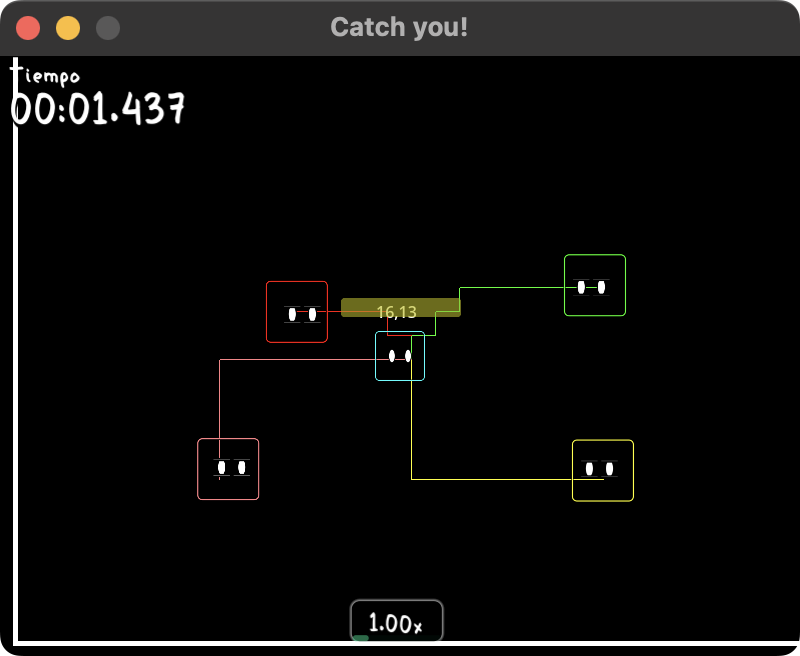
\includegraphics[width = 80mm]{_capt-juego.png}
\end{center}

"Catch You!" es un juego elaborado en Godot 4 donde el jugador, representado por un cubo de color cyan,
debe sobrevivir por la mayor cantidad de tiempo posible, mientras evita 4 enemigos, que son cubos de mayor tamaño que el jugador
y contienen habilidades especiales cada uno. En la esquina superior izquierda se encuentra el tiempo actual,
que representa el tiempo de supervivencia del jugador. Si hay un record existente, se indicará debajo del tiempo una vez que sea alcanzada.

En la parte inferior se encuentra el multiplicador de movimiento. La velocidad de los oponentes es multiplicada con este valor, e incrementa cada 10 segundos.
El jugador no es afectado por esto, y deberá utilizar más su cohete cuando este multiplicador incremente para evitar a los oponentes.

\begin{center}
    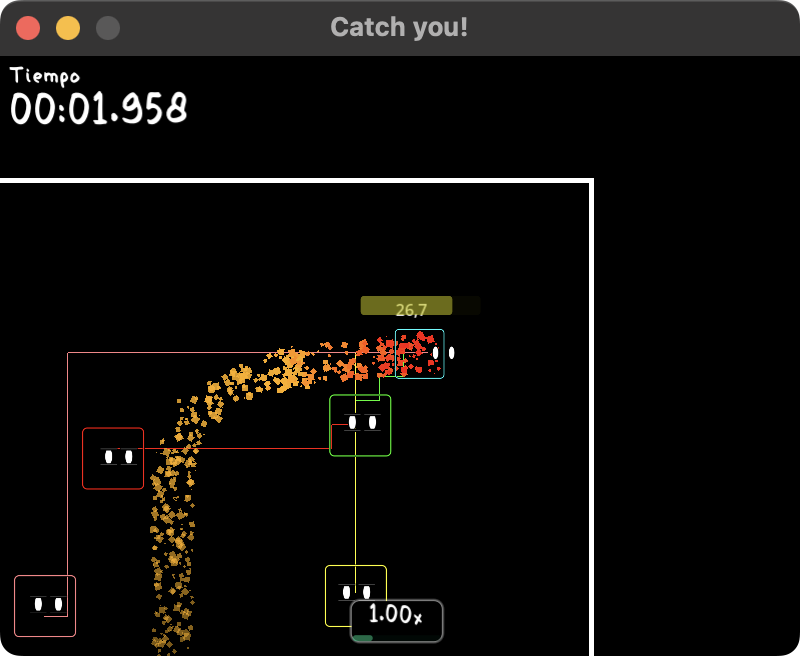
\includegraphics[width = 80mm]{_capt-cohete.png}
\end{center}

El jugador tiene equipado un cohete, que el permite acelerar durante 3 segundos acumulados con una aceleración mayor que le permite
escapar de los oponentes que lo persiguen en el area de juego. El cohete contiene un "cooldown", que es un tiempo donde no realizará una recarga,
y esto es aplicada al momento que el jugador suelte el botón de cohete (Espacio). Este cooldown tiene una duración de 0.3 segundos antes que vuelva a
comenzar el rellenado del cohete. La cantidad restante del cohete es mostrado por una barra amarilla indicada en la parte superior del jugador.

\section{Enemigos y algoritmos}

La siguiente sección visualiza cada enemigo y su funcionalidad y habilidad especial. Cada enemigo es generado por medio de una escena dedicada,
que es instanciada en la escena de juego. Dado su implementación, las acciones que requieran ser enviadas por medio de una señal, son enviadas de manera
manual hacia el nodo principal de juego. Ellos no tienen idea del area de juego; solamente saben que existen en una area y pueden colisionar con otros objetos que existen en el mismo plano que ellos. Dado esto, no se puede
obtener al jugador directamente y verificar, hay que asignar los cuerpos un tipo de llave unica que los defina, por esto el grupo fue asignado.

\lstinputlisting{cod/global-signal-view.gd}

Para realizar este envio, se conecta una instancia global, llamada GlobalVars, donde contiene una señal que cualquier elemento puede enviar. Con esto, se puede conectar
el Nodo de juego con este, y ahora puede recibir mensajes. Cualquier enemigo que necesite enviar el mensaje solamente tiene que enviar el comando para emitir
el mensaje, y Juego lo recibirá.

\lstinputlisting{cod/main-game-ready.gd}

\lstinputlisting{cod/area-hit-code.gd}

Como se muestra en este bloque, al momento que algún enemigo toque a un cuerpo, verificará primero si el cuerpo que haya hecho colisión es parte de un grupo llamado
"player", donde el jugador es el unico asignado. Una vez confirmado que el cuerpo es del grupo "player", emitirá la señal "playerHit", que fue conectada al juego principal y
llamará la función \_onPlayerHit(), que subsequentemente llamará actionLoseGame().

\lstinputlisting{cod/player-hit.gd}

\subsection{Rojo}


\includegraphics[width = 20mm]{_enem-rojo.png}

El cubo rojo contiene la actividad más básica, donde solamente busca la ubicación del jugador por medio del algoritmo Estrella.

\lstinputlisting[caption = Algoritmo del enemigo rojo]{cod/STRNode.gd}

\subsection{Verde}

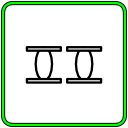
\includegraphics[width = 20mm]{_enem-verde.png}


El cubo verde también busca la ubicación del jugador, pero utiliza el método Greedy para encontrar la posición.
A diferencia del rojo, el cubo verde contiene la habilidad de expandirse después de un tiempo determinado para bloquear
el paso al jugador. Esto puede ser un obstaculo, pero al mismo tiempo puede ser una mecánica a su favor, ya que
el jugador puede utilizar este mismo bloqueo a los otros enemigos, cortandoles el paso y dejandolo escapar.

\lstinputlisting[caption = Algoritmo del enemigo verde]{cod/GRNode.gd}

\lstinputlisting[caption = Funcionalidad de habilidad del enemigo verde.]{cod/Enem2-habilidad.gd}

\subsection{Amarillo}


\includegraphics[width = 20mm]{_enem-amarillo.png}


El cubo amarillo tiene la habilidad de un cohete, que le permite acelerar a una velocidad mayor que el jugador.
Debes de tener cuidado con este si está cerca, si activa su cohete, ¡checa si tienes gasolina suficiente en tu cohete para escapar!

Este cubo utiliza el algoritmo BPA, también conocido como "Breadth-First Search" (BFS).
Dado la manera que fue enseñada este algoritmo, se realizaron cambios que permiten el procedimiento del algoritmo para evitar el problema
con Godot limitando a 1024 el tamaño del stack en una llamada.

\lstinputlisting[caption = Algoritmo del enemigo amarillo]{cod/BFSNode.gd}

\subsection{Naranja}


\includegraphics[width = 20mm]{_enem-naranja.png}

Este cubo utiliza el algoritmo BPP, también conocido como "Depth-First Search", (DFS).

En la versión actual de "Catch You!", el cubo naranja contiene la misma habilidad que el cubo amarillo.
En una actualización futura, se implementará su habilidad especial que permite saltar del mapa y caer en otra posición
aleatoria o calculada por el mismo algoritmo para sorprender al jugador en su trama.

\lstinputlisting[caption = Algoritmo del enemigo naranja]{cod/DFSNode.gd}

\subsection{Conversión para algoritmos BPA y BPP}

Dado la limitación de Godot con un stack de 1024 elementos en una función dada, se tuvo que refactorizar el proceso del algoritmo
para aceptar un número arbitrario de elementos, por lo que el proceso fue cambiado de una función recursiva a una donde involucra un
ciclo while mientras contiene todos los elementos posibles a un "stack", que es un Array de elementos almacenado en la función como memoria
temporal.

Otro cambio realizado para estos algoritmos fue el cambio de la variable de elementos visitados de un Array a un Diccionario. Este tipo de dato
permite agregar y obtener datos por medio de un HashMap, que es una representación unica para cada elemento que permite un lookup más rapido.
Utilizando un Array en estos algoritmos resultaba en ciclo muy grande, que ralentiza el rendimiento del juego de manera exponencial, basado en la cantidad
disponible de bloques en el mapa.

Cada elemento es analizado al diccionario de elementos visitados. Si el elemento no ha sido visitado, se genera los nodos adyacentes y se agregan
al stack para ser procesados.

\lstinputlisting[caption = Codigo de busqueda de busqueda del enemigo amarillo y naranja.]{cod/bps-code.gd}

\section{Procesamiento de posiciones}

Dado que "Catch You!" permite movimiento libre con el jugador, Su posición debe ser generalizada a un vector que lo representa en una especie de cuadrícula.
La clase de GlobalVars contiene una función que realiza esta acción.

\lstinputlisting{cod/titleSet.gd}

Cada enemigo también proveé su posición basado en la cuadrícula, lo que facilita el calculo de los algoritmos por la facilidad de posicionamiento, en vez de calcular
cada número flotante que sea remotamente posible en el area alrededor del enemigo.

\lstinputlisting[caption = Codigo de expansion de busqueda del enemigo verde (Greedy).]{cod/expand-greedy.gd}

\section{Limitaciones}

\subsection{Tamaño del mapa}

Originalmente, el juego incrementaria el tamaño del area del juego lentamente basado en el tiempo. Pero durante la
implementación de los algoritmos BPA y BPP, el proceso de busqueda terminaba analizado cada bloque disponible, que se volveria
peor con las siguientes dos condiciones:
\begin{itemize}
    \item La cantidad de bloques disponibles incrementa mientras crece el mapa.
    \item El jugador se aleja del oponente, haciendo que el resultado final del oponente sea mas largo, por lo tanto
    siendo más costosa mientras encuentra al jugador.
\end{itemize}

\subsection{Margen de busqueda para los algoritmos}

Con la implementación de BPA y BPP ralentizando el juego de manera expotencial cuando se aleje del jugador o cuando crecía el
area de juego, fue necesario aplicar un limite de exploración donde el bloque no pudede hacer calculos de posicionamiento
afuera de esta area. En este caso, son 15 bloques en cada posible dirección del enemigo, creando un margen cuadrado.

\lstinputlisting[caption = Limite de busqueda en la función expand de enemigo 3 y 4.]{cod/exp-limitedfind.gd}

\end{document}